% !TEX TS-program = pdflatex
% !TEX encoding = UTF-8 Unicode
\documentclass[border=0mm]{standalone}
% packages
\usepackage{tikz}
\usetikzlibrary{patterns}
\usepackage{amsmath,amssymb}
\usepackage{bm}
\usepackage{pgfplots}
\pgfplotsset{compat=1.15}
% start document
\begin{document}
% generated by ROOT (CERN)
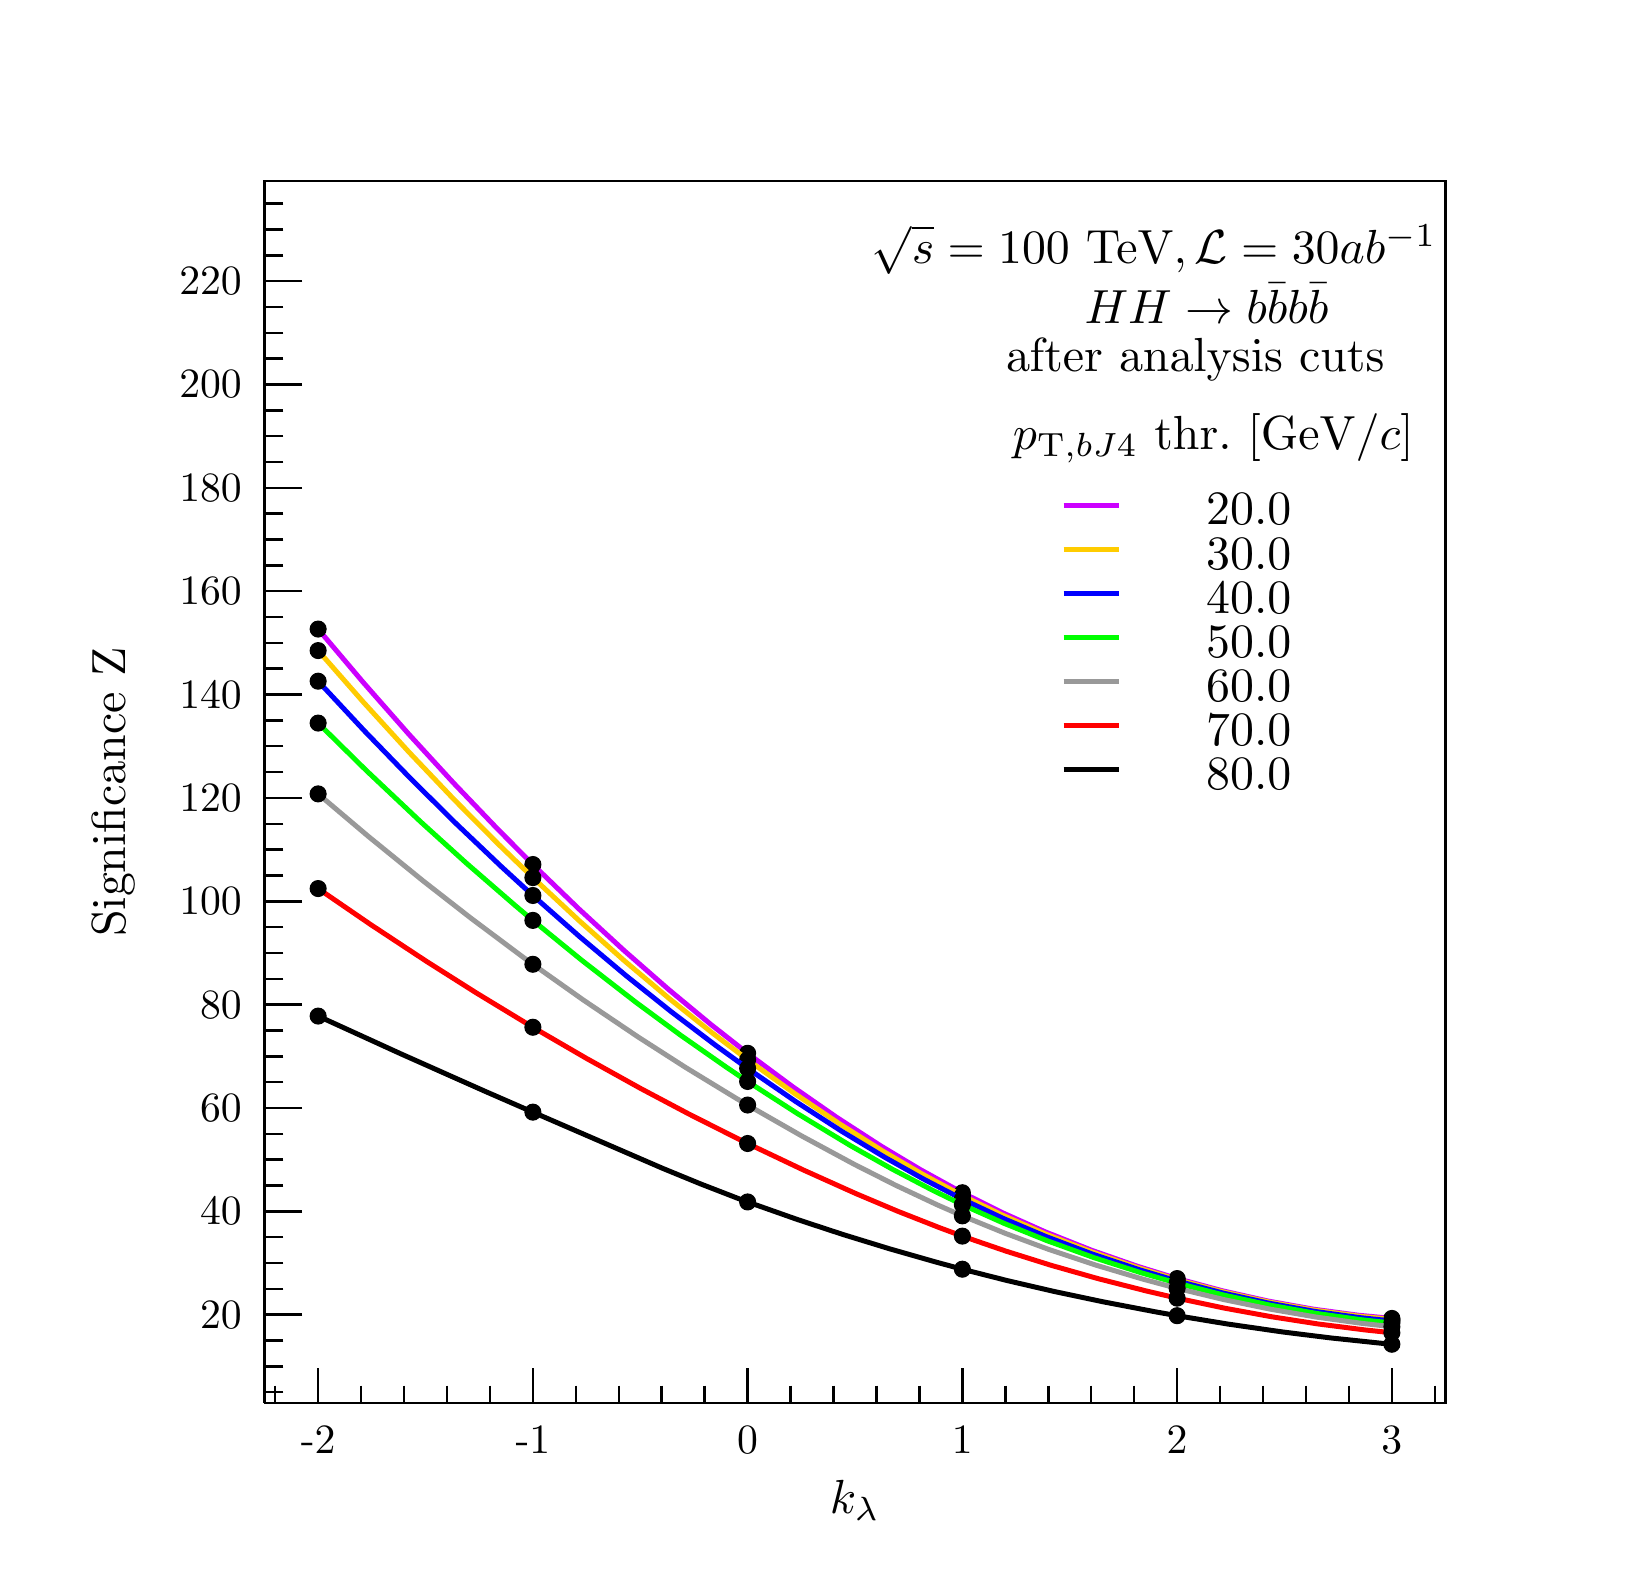
\begin{tikzpicture}
\pgfdeclareplotmark{cross} {
\pgfpathmoveto{\pgfpoint{-0.3\pgfplotmarksize}{\pgfplotmarksize}}
\pgfpathlineto{\pgfpoint{+0.3\pgfplotmarksize}{\pgfplotmarksize}}
\pgfpathlineto{\pgfpoint{+0.3\pgfplotmarksize}{0.3\pgfplotmarksize}}
\pgfpathlineto{\pgfpoint{+1\pgfplotmarksize}{0.3\pgfplotmarksize}}
\pgfpathlineto{\pgfpoint{+1\pgfplotmarksize}{-0.3\pgfplotmarksize}}
\pgfpathlineto{\pgfpoint{+0.3\pgfplotmarksize}{-0.3\pgfplotmarksize}}
\pgfpathlineto{\pgfpoint{+0.3\pgfplotmarksize}{-1.\pgfplotmarksize}}
\pgfpathlineto{\pgfpoint{-0.3\pgfplotmarksize}{-1.\pgfplotmarksize}}
\pgfpathlineto{\pgfpoint{-0.3\pgfplotmarksize}{-0.3\pgfplotmarksize}}
\pgfpathlineto{\pgfpoint{-1.\pgfplotmarksize}{-0.3\pgfplotmarksize}}
\pgfpathlineto{\pgfpoint{-1.\pgfplotmarksize}{0.3\pgfplotmarksize}}
\pgfpathlineto{\pgfpoint{-0.3\pgfplotmarksize}{0.3\pgfplotmarksize}}
\pgfpathclose
\pgfusepathqstroke
}
\pgfdeclareplotmark{cross*} {
\pgfpathmoveto{\pgfpoint{-0.3\pgfplotmarksize}{\pgfplotmarksize}}
\pgfpathlineto{\pgfpoint{+0.3\pgfplotmarksize}{\pgfplotmarksize}}
\pgfpathlineto{\pgfpoint{+0.3\pgfplotmarksize}{0.3\pgfplotmarksize}}
\pgfpathlineto{\pgfpoint{+1\pgfplotmarksize}{0.3\pgfplotmarksize}}
\pgfpathlineto{\pgfpoint{+1\pgfplotmarksize}{-0.3\pgfplotmarksize}}
\pgfpathlineto{\pgfpoint{+0.3\pgfplotmarksize}{-0.3\pgfplotmarksize}}
\pgfpathlineto{\pgfpoint{+0.3\pgfplotmarksize}{-1.\pgfplotmarksize}}
\pgfpathlineto{\pgfpoint{-0.3\pgfplotmarksize}{-1.\pgfplotmarksize}}
\pgfpathlineto{\pgfpoint{-0.3\pgfplotmarksize}{-0.3\pgfplotmarksize}}
\pgfpathlineto{\pgfpoint{-1.\pgfplotmarksize}{-0.3\pgfplotmarksize}}
\pgfpathlineto{\pgfpoint{-1.\pgfplotmarksize}{0.3\pgfplotmarksize}}
\pgfpathlineto{\pgfpoint{-0.3\pgfplotmarksize}{0.3\pgfplotmarksize}}
\pgfpathclose
\pgfusepathqfillstroke
}
\pgfdeclareplotmark{newstar} {
\pgfpathmoveto{\pgfqpoint{0pt}{\pgfplotmarksize}}
\pgfpathlineto{\pgfqpointpolar{44}{0.5\pgfplotmarksize}}
\pgfpathlineto{\pgfqpointpolar{18}{\pgfplotmarksize}}
\pgfpathlineto{\pgfqpointpolar{-20}{0.5\pgfplotmarksize}}
\pgfpathlineto{\pgfqpointpolar{-54}{\pgfplotmarksize}}
\pgfpathlineto{\pgfqpointpolar{-90}{0.5\pgfplotmarksize}}
\pgfpathlineto{\pgfqpointpolar{234}{\pgfplotmarksize}}
\pgfpathlineto{\pgfqpointpolar{198}{0.5\pgfplotmarksize}}
\pgfpathlineto{\pgfqpointpolar{162}{\pgfplotmarksize}}
\pgfpathlineto{\pgfqpointpolar{134}{0.5\pgfplotmarksize}}
\pgfpathclose
\pgfusepathqstroke
}
\pgfdeclareplotmark{newstar*} {
\pgfpathmoveto{\pgfqpoint{0pt}{\pgfplotmarksize}}
\pgfpathlineto{\pgfqpointpolar{44}{0.5\pgfplotmarksize}}
\pgfpathlineto{\pgfqpointpolar{18}{\pgfplotmarksize}}
\pgfpathlineto{\pgfqpointpolar{-20}{0.5\pgfplotmarksize}}
\pgfpathlineto{\pgfqpointpolar{-54}{\pgfplotmarksize}}
\pgfpathlineto{\pgfqpointpolar{-90}{0.5\pgfplotmarksize}}
\pgfpathlineto{\pgfqpointpolar{234}{\pgfplotmarksize}}
\pgfpathlineto{\pgfqpointpolar{198}{0.5\pgfplotmarksize}}
\pgfpathlineto{\pgfqpointpolar{162}{\pgfplotmarksize}}
\pgfpathlineto{\pgfqpointpolar{134}{0.5\pgfplotmarksize}}
\pgfpathclose
\pgfusepathqfillstroke
}
\definecolor{c}{rgb}{1,1,1};
\draw [color=c, fill=c] (0,0) rectangle (20,19.397);
\draw [color=c, fill=c] (3,1.9397) rectangle (18,17.4573);
\definecolor{c}{rgb}{0,0,0};
\draw [c,line width=0.9] (3,1.9397) -- (3,17.4573) -- (18,17.4573) -- (18,1.9397) -- (3,1.9397);
\definecolor{c}{rgb}{1,1,1};
\draw [color=c, fill=c] (3,1.9397) rectangle (18,17.4573);
\definecolor{c}{rgb}{0,0,0};
\draw [c,line width=0.9] (3,1.9397) -- (3,17.4573) -- (18,17.4573) -- (18,1.9397) -- (3,1.9397);
\draw [c,line width=0.9] (3,1.9397) -- (18,1.9397);
\draw [c,line width=0.9] (3.68182,2.37613) -- (3.68182,1.9397);
\draw [c,line width=0.9] (4.22727,2.15791) -- (4.22727,1.9397);
\draw [c,line width=0.9] (4.77273,2.15791) -- (4.77273,1.9397);
\draw [c,line width=0.9] (5.31818,2.15791) -- (5.31818,1.9397);
\draw [c,line width=0.9] (5.86364,2.15791) -- (5.86364,1.9397);
\draw [c,line width=0.9] (6.40909,2.37613) -- (6.40909,1.9397);
\draw [c,line width=0.9] (6.95455,2.15791) -- (6.95455,1.9397);
\draw [c,line width=0.9] (7.5,2.15791) -- (7.5,1.9397);
\draw [c,line width=0.9] (8.04545,2.15791) -- (8.04545,1.9397);
\draw [c,line width=0.9] (8.59091,2.15791) -- (8.59091,1.9397);
\draw [c,line width=0.9] (9.13636,2.37613) -- (9.13636,1.9397);
\draw [c,line width=0.9] (9.68182,2.15791) -- (9.68182,1.9397);
\draw [c,line width=0.9] (10.2273,2.15791) -- (10.2273,1.9397);
\draw [c,line width=0.9] (10.7727,2.15791) -- (10.7727,1.9397);
\draw [c,line width=0.9] (11.3182,2.15791) -- (11.3182,1.9397);
\draw [c,line width=0.9] (11.8636,2.37613) -- (11.8636,1.9397);
\draw [c,line width=0.9] (12.4091,2.15791) -- (12.4091,1.9397);
\draw [c,line width=0.9] (12.9545,2.15791) -- (12.9545,1.9397);
\draw [c,line width=0.9] (13.5,2.15791) -- (13.5,1.9397);
\draw [c,line width=0.9] (14.0455,2.15791) -- (14.0455,1.9397);
\draw [c,line width=0.9] (14.5909,2.37613) -- (14.5909,1.9397);
\draw [c,line width=0.9] (15.1364,2.15791) -- (15.1364,1.9397);
\draw [c,line width=0.9] (15.6818,2.15791) -- (15.6818,1.9397);
\draw [c,line width=0.9] (16.2273,2.15791) -- (16.2273,1.9397);
\draw [c,line width=0.9] (16.7727,2.15791) -- (16.7727,1.9397);
\draw [c,line width=0.9] (17.3182,2.37613) -- (17.3182,1.9397);
\draw [c,line width=0.9] (3.68182,2.37613) -- (3.68182,1.9397);
\draw [c,line width=0.9] (3.13636,2.15791) -- (3.13636,1.9397);
\draw [c,line width=0.9] (17.3182,2.37613) -- (17.3182,1.9397);
\draw [c,line width=0.9] (17.8636,2.15791) -- (17.8636,1.9397);
\draw [anchor=base] (3.68182,1.2996) node[scale=1.50669, color=c, rotate=0]{-2};
\draw [anchor=base] (6.40909,1.2996) node[scale=1.50669, color=c, rotate=0]{-1};
\draw [anchor=base] (9.13636,1.2996) node[scale=1.50669, color=c, rotate=0]{0};
\draw [anchor=base] (11.8636,1.2996) node[scale=1.50669, color=c, rotate=0]{1};
\draw [anchor=base] (14.5909,1.2996) node[scale=1.50669, color=c, rotate=0]{2};
\draw [anchor=base] (17.3182,1.2996) node[scale=1.50669, color=c, rotate=0]{3};
\draw (10.5,0.698292) node[scale=1.7299, color=c, rotate=0]{$k_{\lambda}$};
\draw [c,line width=0.9] (3,1.9397) -- (3,17.4573);
\draw [c,line width=0.9] (3.48,3.05906) -- (3,3.05906);
\draw [c,line width=0.9] (3.24,3.3872) -- (3,3.3872);
\draw [c,line width=0.9] (3.24,3.71533) -- (3,3.71533);
\draw [c,line width=0.9] (3.24,4.04347) -- (3,4.04347);
\draw [c,line width=0.9] (3.48,4.37161) -- (3,4.37161);
\draw [c,line width=0.9] (3.24,4.69975) -- (3,4.69975);
\draw [c,line width=0.9] (3.24,5.02788) -- (3,5.02788);
\draw [c,line width=0.9] (3.24,5.35602) -- (3,5.35602);
\draw [c,line width=0.9] (3.48,5.68416) -- (3,5.68416);
\draw [c,line width=0.9] (3.24,6.0123) -- (3,6.0123);
\draw [c,line width=0.9] (3.24,6.34043) -- (3,6.34043);
\draw [c,line width=0.9] (3.24,6.66857) -- (3,6.66857);
\draw [c,line width=0.9] (3.48,6.99671) -- (3,6.99671);
\draw [c,line width=0.9] (3.24,7.32485) -- (3,7.32485);
\draw [c,line width=0.9] (3.24,7.65298) -- (3,7.65298);
\draw [c,line width=0.9] (3.24,7.98112) -- (3,7.98112);
\draw [c,line width=0.9] (3.48,8.30926) -- (3,8.30926);
\draw [c,line width=0.9] (3.24,8.63739) -- (3,8.63739);
\draw [c,line width=0.9] (3.24,8.96553) -- (3,8.96553);
\draw [c,line width=0.9] (3.24,9.29367) -- (3,9.29367);
\draw [c,line width=0.9] (3.48,9.62181) -- (3,9.62181);
\draw [c,line width=0.9] (3.24,9.94994) -- (3,9.94994);
\draw [c,line width=0.9] (3.24,10.2781) -- (3,10.2781);
\draw [c,line width=0.9] (3.24,10.6062) -- (3,10.6062);
\draw [c,line width=0.9] (3.48,10.9344) -- (3,10.9344);
\draw [c,line width=0.9] (3.24,11.2625) -- (3,11.2625);
\draw [c,line width=0.9] (3.24,11.5906) -- (3,11.5906);
\draw [c,line width=0.9] (3.24,11.9188) -- (3,11.9188);
\draw [c,line width=0.9] (3.48,12.2469) -- (3,12.2469);
\draw [c,line width=0.9] (3.24,12.575) -- (3,12.575);
\draw [c,line width=0.9] (3.24,12.9032) -- (3,12.9032);
\draw [c,line width=0.9] (3.24,13.2313) -- (3,13.2313);
\draw [c,line width=0.9] (3.48,13.5595) -- (3,13.5595);
\draw [c,line width=0.9] (3.24,13.8876) -- (3,13.8876);
\draw [c,line width=0.9] (3.24,14.2157) -- (3,14.2157);
\draw [c,line width=0.9] (3.24,14.5439) -- (3,14.5439);
\draw [c,line width=0.9] (3.48,14.872) -- (3,14.872);
\draw [c,line width=0.9] (3.24,15.2001) -- (3,15.2001);
\draw [c,line width=0.9] (3.24,15.5283) -- (3,15.5283);
\draw [c,line width=0.9] (3.24,15.8564) -- (3,15.8564);
\draw [c,line width=0.9] (3.48,16.1846) -- (3,16.1846);
\draw [c,line width=0.9] (3.48,3.05906) -- (3,3.05906);
\draw [c,line width=0.9] (3.24,2.73092) -- (3,2.73092);
\draw [c,line width=0.9] (3.24,2.40278) -- (3,2.40278);
\draw [c,line width=0.9] (3.24,2.07465) -- (3,2.07465);
\draw [c,line width=0.9] (3.48,16.1846) -- (3,16.1846);
\draw [c,line width=0.9] (3.24,16.5127) -- (3,16.5127);
\draw [c,line width=0.9] (3.24,16.8408) -- (3,16.8408);
\draw [c,line width=0.9] (3.24,17.169) -- (3,17.169);
\draw [anchor= east] (2.9,3.05906) node[scale=1.50669, color=c, rotate=0]{20};
\draw [anchor= east] (2.9,4.37161) node[scale=1.50669, color=c, rotate=0]{40};
\draw [anchor= east] (2.9,5.68416) node[scale=1.50669, color=c, rotate=0]{60};
\draw [anchor= east] (2.9,6.99671) node[scale=1.50669, color=c, rotate=0]{80};
\draw [anchor= east] (2.9,8.30926) node[scale=1.50669, color=c, rotate=0]{100};
\draw [anchor= east] (2.9,9.62181) node[scale=1.50669, color=c, rotate=0]{120};
\draw [anchor= east] (2.9,10.9344) node[scale=1.50669, color=c, rotate=0]{140};
\draw [anchor= east] (2.9,12.2469) node[scale=1.50669, color=c, rotate=0]{160};
\draw [anchor= east] (2.9,13.5595) node[scale=1.50669, color=c, rotate=0]{180};
\draw [anchor= east] (2.9,14.872) node[scale=1.50669, color=c, rotate=0]{200};
\draw [anchor= east] (2.9,16.1846) node[scale=1.50669, color=c, rotate=0]{220};
\draw (1.08,9.69849) node[scale=1.7299, color=c, rotate=90]{Significance Z};
\definecolor{c}{rgb}{0.8,0,1};
\draw [c,line width=1.8] (3.68182,11.7662) -- (4.2547,11.0888) -- (4.83154,10.4333) -- (5.4059,9.80692) -- (5.96507,9.22242) -- (6.40909,8.77604) -- (6.99361,8.2117) -- (7.57061,7.68071) -- (8.13262,7.1894) -- (8.66543,6.74806) -- (9.13636,6.37843)
 -- (9.70783,5.95456) -- (10.2693,5.56399) -- (10.8242,5.20464) -- (11.3273,4.90284) -- (11.8636,4.60759) -- (12.3784,4.35117) -- (12.9154,4.11111) -- (13.5097,3.87542) -- (14.0891,3.67317) -- (14.5909,3.51781) -- (15.1686,3.36187) --
 (15.7496,3.23146) -- (16.3252,3.12835) -- (16.8899,3.05244) -- (17.3182,3.01153);
\definecolor{c}{rgb}{0,0,0};
\foreach \P in {(3.68182,11.7662), (6.40909,8.77604), (9.13636,6.37843), (11.8636,4.60759), (14.5909,3.51781), (17.3182,3.01153)}{\draw[mark options={color=c,fill=c},mark size=2.882883pt,mark=*] plot coordinates {\P};}
\definecolor{c}{rgb}{1,0.8,0};
\draw [c,line width=1.8] (3.68182,11.493) -- (4.25731,10.837) -- (4.83644,10.2026) -- (5.41151,9.5981) -- (5.97393,9.03149) -- (6.40909,8.60973) -- (6.99116,8.06795) -- (7.57071,7.55399) -- (8.13895,7.07525) -- (8.68703,6.63758) -- (9.13636,6.29671)
 -- (9.7259,5.87258) -- (10.2962,5.48715) -- (10.8458,5.14084) -- (11.3469,4.84807) -- (11.8636,4.57063) -- (12.378,4.32048) -- (12.9154,4.0857) -- (13.5111,3.85459) -- (14.0946,3.65503) -- (14.5909,3.50406) -- (15.1713,3.34954) -- (15.7546,3.21986)
 -- (16.331,3.11692) -- (16.8991,3.03999) -- (17.3182,2.99885);
\definecolor{c}{rgb}{0,0,0};
\foreach \P in {(3.68182,11.493), (6.40909,8.60973), (9.13636,6.29671), (11.8636,4.57063), (14.5909,3.50406), (17.3182,2.99885)}{\draw[mark options={color=c,fill=c},mark size=2.882883pt,mark=*] plot coordinates {\P};}
\definecolor{c}{rgb}{0,0,1};
\draw [c,line width=1.8] (3.68182,11.1041) -- (4.2695,10.4732) -- (4.8593,9.86464) -- (5.43826,9.29118) -- (6.0161,8.74244) -- (6.40909,8.38272) -- (7.00186,7.8605) -- (7.59203,7.36498) -- (8.16553,6.90712) -- (8.73236,6.47787) -- (9.13636,6.18624)
 -- (9.74767,5.76579) -- (10.3293,5.38934) -- (10.8744,5.05979) -- (11.3776,4.77722) -- (11.8636,4.52574) -- (12.3829,4.2814) -- (12.9246,4.05192) -- (13.5204,3.82707) -- (14.1077,3.63103) -- (14.5909,3.48689) -- (15.1745,3.33367) --
 (15.7606,3.20427) -- (16.338,3.10079) -- (16.9102,3.02174) -- (17.3182,2.97965);
\definecolor{c}{rgb}{0,0,0};
\foreach \P in {(3.68182,11.1041), (6.40909,8.38272), (9.13636,6.18624), (11.8636,4.52574), (14.5909,3.48689), (17.3182,2.97965)}{\draw[mark options={color=c,fill=c},mark size=2.882883pt,mark=*] plot coordinates {\P};}
\definecolor{c}{rgb}{0,1,0};
\draw [c,line width=1.8] (3.68182,10.5723) -- (4.2913,9.97225) -- (4.98823,9.31439) -- (5.57031,8.788) -- (6.18114,8.25818) -- (6.40909,8.06638) -- (7.02779,7.56155) -- (7.71905,7.02511) -- (8.28774,6.60633) -- (8.87607,6.19517) -- (9.13636,6.0206)
 -- (9.76721,5.61401) -- (10.4433,5.20525) -- (10.9731,4.90702) -- (11.4874,4.63813) -- (11.8636,4.45535) -- (12.3903,4.21992) -- (12.9389,3.99855) -- (13.5359,3.78308) -- (14.1313,3.59213) -- (14.5909,3.45951) -- (15.1808,3.30844) --
 (15.7724,3.17989) -- (16.3521,3.07624) -- (16.9322,2.9946) -- (17.3182,2.95253);
\definecolor{c}{rgb}{0,0,0};
\foreach \P in {(3.68182,10.5723), (6.40909,8.06638), (9.13636,6.0206), (11.8636,4.45535), (14.5909,3.45951), (17.3182,2.95253)}{\draw[mark options={color=c,fill=c},mark size=2.882883pt,mark=*] plot coordinates {\P};}
\definecolor{c}{rgb}{0.6,0.6,0.6};
\draw [c,line width=1.8] (3.68182,9.6728) -- (4.31831,9.13411) -- (5.01803,8.5656) -- (5.62151,8.09521) -- (6.25887,7.61843) -- (6.40909,7.50904) -- (7.04854,7.05611) -- (7.7466,6.58517) -- (8.34612,6.20046) -- (8.97801,5.8149) -- (9.13636,5.7215) --
 (9.82581,5.32724) -- (10.4907,4.96836) -- (11.0187,4.70146) -- (11.5385,4.45679) -- (11.8636,4.31392) -- (12.407,4.09253) -- (12.9667,3.88557) -- (13.5594,3.68821) -- (14.1515,3.51182) -- (14.5909,3.39341) -- (15.1811,3.25131) -- (15.773,3.12919) --
 (16.3528,3.02937) -- (16.9333,2.94903) -- (17.3182,2.9066);
\definecolor{c}{rgb}{0,0,0};
\foreach \P in {(3.68182,9.6728), (6.40909,7.50904), (9.13636,5.7215), (11.8636,4.31392), (14.5909,3.39341), (17.3182,2.9066)}{\draw[mark options={color=c,fill=c},mark size=2.882883pt,mark=*] plot coordinates {\P};}
\definecolor{c}{rgb}{1,0,0};
\draw [c,line width=1.8] (3.68182,8.47067) -- (4.35014,8.01261) -- (5.05582,7.54757) -- (5.68972,7.14613) -- (6.40909,6.70924) -- (7.0879,6.3148) -- (7.78517,5.92778) -- (8.39805,5.60337) -- (9.03774,5.2811) -- (9.13636,5.23293) -- (9.84726,4.89518)
 -- (10.5108,4.59701) -- (11.045,4.37165) -- (11.5784,4.16182) -- (11.8636,4.05657) -- (12.4206,3.86483) -- (12.9929,3.68532) -- (13.5892,3.51601) -- (14.1972,3.3607) -- (14.5909,3.26887) -- (15.1933,3.14185) -- (15.7959,3.03176) -- (16.3807,2.94116)
 -- (16.9769,2.86528) -- (17.3182,2.82933);
\definecolor{c}{rgb}{0,0,0};
\foreach \P in {(3.68182,8.47067), (6.40909,6.70924), (9.13636,5.23293), (11.8636,4.05657), (14.5909,3.26887), (17.3182,2.82933)}{\draw[mark options={color=c,fill=c},mark size=2.882883pt,mark=*] plot coordinates {\P};}
\draw [c,line width=1.8] (3.68182,6.85119) -- (4.7319,6.37194) -- (5.80388,5.8949) -- (6.40909,5.63102) -- (8.05868,4.91676) -- (8.53886,4.71982) -- (9.01029,4.53722) -- (9.13636,4.49061) -- (9.77547,4.26526) -- (10.3499,4.07644) -- (10.9314,3.8979)
 -- (11.5333,3.72573) -- (11.8636,3.63646) -- (12.4357,3.49141) -- (13.0328,3.35296) -- (13.654,3.22182) -- (14.3199,3.0944) -- (14.5909,3.0461) -- (15.2329,2.94028) -- (15.9334,2.8392) -- (16.5415,2.76365) -- (17.1833,2.69618) -- (17.3182,2.68361);
\foreach \P in {(3.68182,6.85119), (6.40909,5.63102), (9.13636,4.49061), (11.8636,3.63646), (14.5909,3.0461), (17.3182,2.68361)}{\draw[mark options={color=c,fill=c},mark size=2.882883pt,mark=*] plot coordinates {\P};}
\draw [anchor=north] (15.05,14.7137) node[scale=1.7299, color=c, rotate=0]{$p_{\text{T}, bJ4} \text{~thr.} ~[\text{GeV}/c]$};
\draw [anchor=base] (15.5,13.649) node[scale=1.7299, color=c, rotate=0]{ };
\draw [anchor=base] (15.5,13.0887) node[scale=1.7299, color=c, rotate=0]{20.0};
\definecolor{c}{rgb}{0.8,0,1};
\draw [c,line width=1.8] (13.15,13.3408) -- (13.85,13.3408);
\definecolor{c}{rgb}{0,0,0};
\draw [anchor=base] (15.5,12.5283) node[scale=1.7299, color=c, rotate=0]{30.0};
\definecolor{c}{rgb}{1,0.8,0};
\draw [c,line width=1.8] (13.15,12.7805) -- (13.85,12.7805);
\definecolor{c}{rgb}{0,0,0};
\draw [anchor=base] (15.5,11.9679) node[scale=1.7299, color=c, rotate=0]{40.0};
\definecolor{c}{rgb}{0,0,1};
\draw [c,line width=1.8] (13.15,12.2201) -- (13.85,12.2201);
\definecolor{c}{rgb}{0,0,0};
\draw [anchor=base] (15.5,11.4076) node[scale=1.7299, color=c, rotate=0]{50.0};
\definecolor{c}{rgb}{0,1,0};
\draw [c,line width=1.8] (13.15,11.6597) -- (13.85,11.6597);
\definecolor{c}{rgb}{0,0,0};
\draw [anchor=base] (15.5,10.8472) node[scale=1.7299, color=c, rotate=0]{60.0};
\definecolor{c}{rgb}{0.6,0.6,0.6};
\draw [c,line width=1.8] (13.15,11.0994) -- (13.85,11.0994);
\definecolor{c}{rgb}{0,0,0};
\draw [anchor=base] (15.5,10.2869) node[scale=1.7299, color=c, rotate=0]{70.0};
\definecolor{c}{rgb}{1,0,0};
\draw [c,line width=1.8] (13.15,10.539) -- (13.85,10.539);
\definecolor{c}{rgb}{0,0,0};
\draw [anchor=base] (15.5,9.72651) node[scale=1.7299, color=c, rotate=0]{80.0};
\draw [c,line width=1.8] (13.15,9.97867) -- (13.85,9.97867);
\draw [anchor= west] (10.5,16.5844) node[scale=1.7299, color=c, rotate=0]{$\sqrt{s} = 100 ~\text{TeV}, \mathcal{L} = 30 ab^{-1}$};
\draw [anchor= west] (13.2,15.9055) node[scale=1.7299, color=c, rotate=0]{$HH \rightarrow b\bar{b}b\bar{b}$};
\draw [anchor=base west] (12.2,15.0424) node[scale=1.7299, color=c, rotate=0]{after analysis cuts};
\end{tikzpicture}
% end document
\end{document}
